\begin{abox}
	Assignment-S05\\
	\vspace{0.5cm}
	Biot Savart Law, Amperes Law and Magnetic Force
	\end{abox}
\begin{enumerate}
	\item $\left. \right. $
	\begin{answer}$\left. \right. $
		\begin{figure}[H]
			\centering
			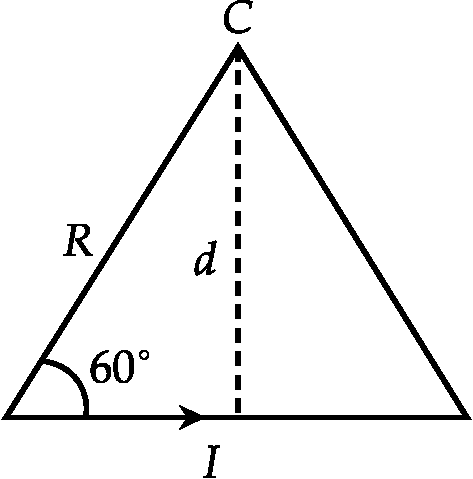
\includegraphics[height=3.5cm,width=3.5cm]{Assi-S20}
		\end{figure}
		\begin{align*}
		d&=R \cos 30^{\circ}=\frac{\sqrt{3}}{2} R\\
		\because B&=\frac{\mu_{0} I}{4 \pi d}\left(\sin \theta_{2}-\sin \theta_{1}\right) \\
		\Rightarrow B_{1}&=\frac{\mu_{0} I}{4 \pi d} 2 \sin 30^{\circ}=\frac{\mu_{0} I}{4 \pi \frac{\sqrt{3}}{2} R} 2 \sin 30^{\circ}=\frac{\mu_{0} I}{2 \sqrt{3} \pi R} \\
		\Rightarrow B&=6 B_{1}=6 \times \frac{\mu_{0} I}{2 \sqrt{3} \pi R}=\frac{3 \mu_{0} I}{\sqrt{3} \pi R}=\frac{\sqrt{3} \mu_{0} I}{\pi R}
		\end{align*}
	\end{answer}
	\item $\left. \right. $
	\begin{answer}
		 Take a point $(x, 0,0)$ on the $x$-axis.
		\begin{align*}
		\text{At this point the magnetic field due to the wire along $\hat{z}$ is} \vec{B}_{1}&=\frac{\mu_{0} I}{2 \pi x} \hat{y}.\\
	\text{	Due to the wire crossing the first and third quadrants is} \vec{B}_{2}&=\frac{\mu_{0} I}{2 \pi x \sin 45^{\circ}} \hat{y}.\\
	\text{	Due to the wire crossing the second and fourth quadrants is} \vec{B}_{3}&=\frac{\mu_{0} I}{2 \pi x \sin 45^{\circ}} \hat{y}.\\
	\text{	Thus, the net magnetic field at point $(x, 0,0)$ is }\vec{B}&=\frac{\mu_{0} I}{2 \pi x}(1+2 \sqrt{2}) \hat{y}.
		\end{align*}
	\end{answer}
	\item $\left. \right. $
	\begin{answer}
		$\left. \right. $
		\begin{figure}[H]
			\centering
			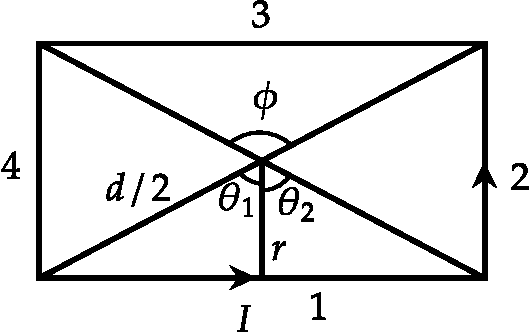
\includegraphics[height=3cm,width=5cm]{Assi-S21}
		\end{figure}
		\begin{align*}
		\because B&=\frac{\mu_{0} I}{4 \pi r}\left(\sin \theta_{2}-\sin \theta_{1}\right)\\
		\text{where }\theta_{1}&=-\frac{\phi}{2}\text{ and }\theta_{2}=\frac{\phi}{2}
	\intertext{	Magnetic field due to segment 1 and 3 is}
		B_{1}&=B_{3}=\frac{\mu_{0} I}{4 \pi(d / 2) \cos \frac{\phi}{2}}\left(\sin \frac{\phi}{2}+\sin \frac{\phi}{2}\right)
	\intertext{	Magnetic field due to segment 2 and 4 is}
		B_{2}&=B_{4}=\frac{\mu_{0} I}{4 \pi(d / 2) \sin \frac{\phi}{2}}\left(\cos \frac{\phi}{2}+\cos \frac{\phi}{2}\right)
	\intertext{	Hence, the magnitude of total magnetic field is}
		B&=B_{1}+B_{2}+B_{3}+B_{4}=\frac{2 \mu_{0} I}{4 \pi(d / 2) \sin \frac{\phi}{2}}\left(\cos \frac{\phi}{2}+\cos \frac{\phi}{2}\right)+\frac{2 \mu_{0} I}{4 \pi(d / 2) \cos \frac{\phi}{2}}\left(\sin \frac{\phi}{2}+\sin \frac{\phi}{2}\right) \\
		B&=\frac{2 \mu_{0} I}{4 \pi(d / 2) \sin \frac{\phi}{2} \cos \frac{\phi}{2}}\left[\left(\cos \frac{\phi}{2}+\cos \frac{\phi}{2}\right) \cos \frac{\phi}{2}+\sin \frac{\phi}{2}\left(\sin \frac{\phi}{2}+\sin \frac{\phi}{2}\right)\right] \\
		B&=\frac{4 \mu_{0} I}{4 \pi(d / 2)}\left[\frac{\cos \frac{\phi}{2}}{\sin \frac{\phi}{2}}+\frac{\sin \frac{\phi}{2}}{\cos \frac{\phi}{2}}\right]=\frac{\mu_{0} I}{\pi(d / 2)}\left[\frac{\cos ^{2} \frac{\phi}{2}+\sin ^{2} \frac{\phi}{2}}{\sin \frac{\phi}{2} \cos \frac{\phi}{2}}\right]=\frac{4 \mu_{0} I}{\pi d \sin \phi}
		\end{align*}
	\end{answer}
	\item $\left. \right. $
	\begin{answer}
		\begin{align*}
		\text{(a) }B&=\frac{\mu_{0} I}{2} \frac{R^{2}}{\left(R^{2}+R^{2}\right)^{3 / 2}}=\frac{\mu_{0} I}{2} \frac{R^{2}}{\left(2 R^{2}\right)^{3 / 2}}\\&=\frac{\mu_{0} I}{4 \sqrt{2} R}=\frac{\mu_{0} \lambda \omega}{4 \sqrt{2}} \because I=\lambda v=\lambda R \omega\\
	\text{	(b) }B&=\frac{\mu_{0} I}{2 R} \Rightarrow B=\frac{\mu_{0} \lambda \omega}{2}\\
		\because I&=\lambda v=\lambda R \omega
		\end{align*}
	\end{answer}
	\item $\left. \right. $
	\begin{answer}
		$$
		\begin{aligned}
	\because B&=\frac{\mu_{0} I}{2} \frac{R^{2}}{\left(R^{2}+d^{2}\right)^{\frac{3}{2}}} \Rightarrow B_{1}=\frac{\mu_{0} I}{2} \frac{R^{2}}{\left(R^{2}+\frac{R^{2}}{4}\right)^{\frac{3}{2}}}, B_{2}=\frac{\mu_{0} I}{2} \frac{R^{2}}{\left(R^{2}+\frac{R^{2}}{4}\right)^{\frac{3}{2}}} \because d=\frac{R}{2}\\
		B&=B_{1}+B_{2}=\frac{\mu_{0} I}{2} \frac{2}{R\left(\frac{5}{4}\right)^{\frac{3}{2}}} \Rightarrow B=\frac{\mu_{0} I 4^{\frac{3}{2}}}{R \quad 5^{\frac{3}{2}}}=\frac{8 \mu_{0} I}{5 \sqrt{5} R}
	\end{aligned}
	$$
	\end{answer}
	\item $\left. \right. $
	\begin{answer}
		\begin{align*}
		\because \oint_{C} \vec{B} \cdot \overrightarrow{d l}&=\mu_{0} I_{e n c} \Rightarrow I_{1}+I_{2}=2, I_{2}+I_{3}=4, I_{1}+I_{2}+I_{3}=1\\
		\Rightarrow I_{1}&=-3 \mathrm{~A}, I_{2}=5 \mathrm{~A}\text{ and }I_{3}=-1 \mathrm{~A} .\\
		I_{1}&=3 A\text{ into the paper, }I_{2}=5 A\text{ out of the paper and }I_{3}=1 A\text{ into the paper}
		\end{align*}
	\end{answer}
	\item $\left. \right. $
	\begin{answer}
			$\left. \right. $
		\begin{figure}[H]
			\centering
			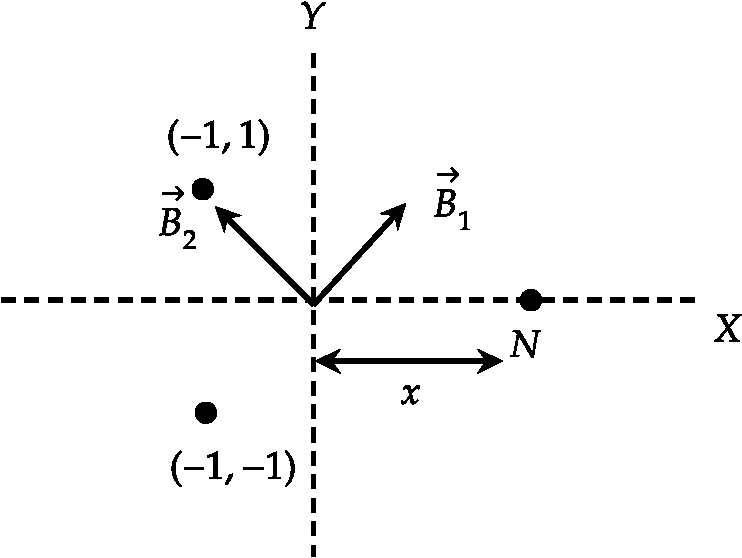
\includegraphics[height=4.5cm,width=5.5cm]{Assi-S22}
		\end{figure}
		\begin{align*}
\text{	(a) }\oint \vec{B} \cdot d \vec{l}&=\mu_{0} I_{e n c}=2 \mu_{0} I\\
		\text{(b) }\left|\vec{B}_{1}\right|&=\left|\vec{B}_{2}\right|=\frac{\mu_{0} I}{2 \sqrt{2} \pi}\\
		\text{Resultant of }&\vec{B}_{1}, \vec{B}_{2}\text{ is}\\
		|\vec{B}|&=\sqrt{2} \frac{\mu_{0} I}{2 \sqrt{2} \pi}=\frac{\mu_{0} I}{2 \pi} \text{(along $y$ direction)}
	\intertext{	The current in the third wire is inward so that }
	\frac{\mu_{0} I}{2 \pi}+\frac{\mu_{0} I}{2 \pi x}&=2 \times \frac{\mu_{0} I}{2 \pi} \Rightarrow x=1 .
		\end{align*}
	\end{answer}
	\item $\left. \right. $
	\begin{answer}
		\begin{align*}
		\text{ Recall Ampere's Law, }\oint_{C} \vec{B} \cdot \overrightarrow{d l}&=\mu_{0} I_{e n c}.
		\end{align*}
			Thus, the field from each conductor is\\
		$B(2 \pi r)=\mu_{0} J \pi R^{2}$, where, $I_{e n c}=J \pi R^{2}$ and $R$ is the radius of the conductor.\\
		(This is a good approximation of the current, as one assumes that the vacuum region in the center is small compared to the area of the conductors.)
		\begin{align*}
		\Rightarrow B&=\frac{\mu_{0} J \pi R^{2}}{2 \pi R}=\frac{\mu_{0} J R}{2}
		\end{align*}
			Making the approximation that $R \approx d / 2$, one has $B \approx \frac{\mu_{0} J d}{4}$\\
		Since both fields contribute in the center, the field is twice that, $\frac{\mu_{0} J d}{2} \hat{y}$.
	\end{answer}
	\item $\left. \right. $
	\begin{answer}
			$\left. \right. $
		\begin{figure}[H]
			\centering
			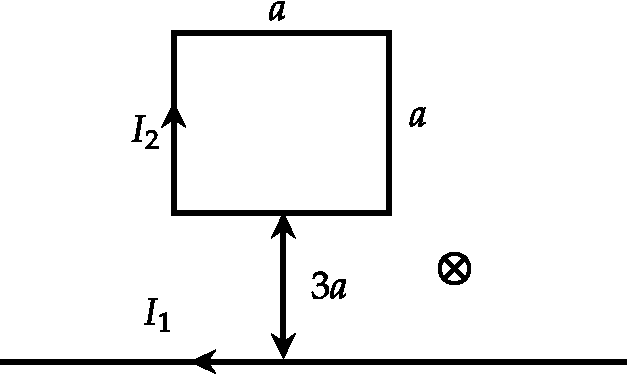
\includegraphics[height=4cm,width=5.8cm]{Assi-S23}
		\end{figure}
		The force on the two sides cancels.
		\begin{align*}
		\text{At the bottom, }B&=\frac{\mu_{0} I_{1}}{2 \pi(3 a)}\\
		\Rightarrow \mathrm{F}&=\left(\frac{\mu_{0} \mathrm{I}_{1}}{6 \pi \mathrm{a}}\right) \mathrm{I}_{2} \mathrm{a}=\frac{\mu_{0} \mathrm{I}_{1} \mathrm{I}_{2}}{6 \pi}(\text { down })\\
	\text{	At the top, }\mathrm{B}&=\frac{\mu_{0} \mathrm{I}_{1}}{2 \pi(3 \mathrm{a}+\mathrm{a})} \Rightarrow \mathrm{F}=\frac{\mu_{0} \mathrm{I}_{1} \mathrm{I}_{2} \mathrm{a}}{8 \pi \mathrm{a}} \Rightarrow \mathrm{F}=\frac{\mu_{0} \mathrm{I}_{1} \mathrm{I}_{2}}{8 \pi}(\text{ up })\\
	 \text{Thus Net Force }&=\left(\frac{\mu_{0} I_{1} I_{2}}{6 \pi}-\frac{\mu_{0} I_{1} I_{2}}{8 \pi}\right)=\frac{\mu_{0} I_{1} I_{2}}{24 \pi}(\text{ down })
		\end{align*}
	\end{answer}
	\item $\left. \right. $
	\begin{answer}
			 (a) The magnetic field at $O$ is only due to the curved path, as for the line element, $d \vec{l} \| \vec{r}$.
			 	\begin{figure}[H]
			 	\centering
			 	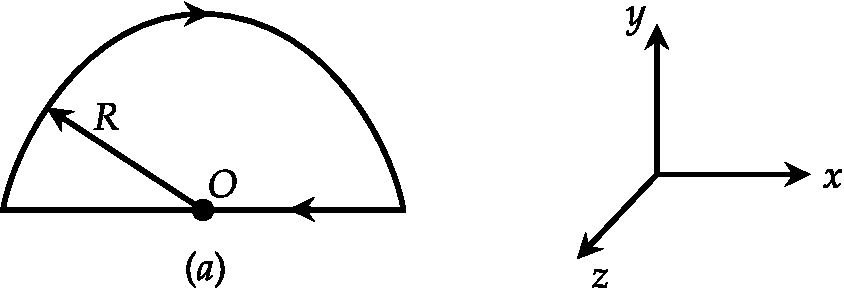
\includegraphics[height=2.5cm,width=6.5cm]{Assi-S24}
			 \end{figure}
		\begin{align*}
	\text{	Hence }\vec{B}&=\frac{\mu_{0} I}{4 R}(-\hat{z}).\\
\text{	Force per unit length }&=I B(-\hat{y})=\frac{\mu_{0} I^{2}}{4 R}(-\hat{y})
	\because \vec{F}=I \int_{\text {line }}(d \vec{l} \times \vec{B})\\
	\text{Magnitude of force per unit length is }\frac{\mu_{0} I^{2}}{4 R}&=\frac{4 \pi \times 10^{-7}(8)^{2}}{4(0.1)}=0.02 \mathrm{~N} / \mathrm{m}
		\end{align*}
		(b) In this part, the magnetic field at $O$ will be effective only due to semi infinite segments of wire. Hence
			\begin{figure}[H]
			\centering
			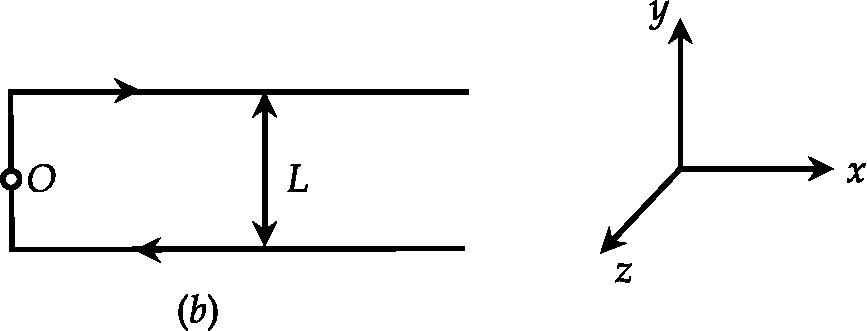
\includegraphics[height=2.5cm,width=6cm]{Assi-S25}
		\end{figure}
			\begin{align*}
		\text{	Hence }\vec{B}&=2 \frac{\mu_{0} I}{4 \pi(l / 2)} \sin \frac{\pi}{2}(-\hat{z})=\frac{\mu_{0} I}{\pi l}(-\hat{z}).\\
		\text{Force per unit length }&=I B(-\hat{x})=\frac{\mu_{0} I^{2}}{\pi l}(-\hat{x}) \quad \because \vec{F}=I \int_{\text {line }}(d \vec{l} \times \vec{B})\\
	\text{	Magnitude of force per unit length is }\frac{\mu_{0} I^{2}}{\pi l}&=\frac{4 \pi \times 10^{-7}(8)^{2}}{\pi(0.2)}=0.13 \mathrm{mN} / \mathrm{m}
			\end{align*}
	\end{answer}
	
	
	
	
\end{enumerate}